% This is a LaTeX thesis template for Adam Mickiewicz University.
% to be used with Rmarkdown
% This template was produced by Jakub Nowosad
% Version: 16 February 2020

% Inspired by:
% This is a LaTeX thesis template for Monash University.
% to be used with Rmarkdown
% This template was produced by Rob Hyndman
% Version: 6 September 2016

\documentclass{amuthesis}
% \usepackage[polish]{babel}
\usepackage{polski}
\renewcommand{\figurename}{Rycina} % Redefine default figure caption %
\renewcommand{\tablename}{Tabela} % Redefine default table caption %
%%%%%%%%%%%%%%%%%%%%%%%%%%%%%%%%%%%%%%%%%%%%%%%%%%%%%%%%%%%%%%%
% Add any LaTeX packages and other preamble here if required
%%%%%%%%%%%%%%%%%%%%%%%%%%%%%%%%%%%%%%%%%%%%%%%%%%%%%%%%%%%%%%%
\usepackage{booktabs,tabularx} % Allows kableExtra to work %
\usepackage{indentfirst} % Adds indent in the first paragraph %
\usepackage{bookmark} % Adds indent in the first paragraph %

\author{Błażej Kościański}
\title{Porównanie metod określania zmian struktury przestrzennej w
kontekście analiz zmian kategorii pokrycia terenu}
\def\titleeng{Comparison of methods for determining changes in spatial
patterns in the context of land cover change analyzes}
\def\degreetitle{Praca magisterska}
\def\major{Geoinformacja}
\def\albumid{444861}
\def\thesisyear{2023}

% Add subject and keywords below
\hypersetup{
     %pdfsubject={The Subject},
     %pdfkeywords={Some Keywords},
     pdfauthor={Błażej Kościański},
     pdftitle={Porównanie metod określania zmian struktury przestrzennej
w kontekście analiz zmian kategorii pokrycia terenu},
     pdfproducer={quarto with LaTeX}
}

\bibliography{thesis.bibpackages.bib}

\begin{document}

\pagenumbering{arabic}

\titlepage

\bookmarksetup{startatroot}

\hypertarget{streszczenie}{%
\chapter*{Streszczenie}\label{streszczenie}}
\addcontentsline{toc}{chapter}{Streszczenie}

\markboth{Streszczenie}{Streszczenie}

\textbf{Abstrakt}

Słowa kluczowe: zmiany pokrycia terenu, struktura przestrzenna, miary
odległości, miary niepodobieństwa, ekologia krajobrazu

\textbf{Abstract}

The abstract must be consistent with the above text.

Keywords: land cover changes, spatial pattern, distance measures,
dissimilarity measures, landscape ecology

\newpage

\setstretch{1.2}\sf\tighttoc\doublespacing

\bookmarksetup{startatroot}

\hypertarget{sec-wprowadzenie}{%
\chapter{Wprowadzenie}\label{sec-wprowadzenie}}

Informacje geograficzne są wynikiem selekcji i przetwarzania danych
związanych z otaczającą nas przestrzenią geograficzną. Pozwalają na
bardziej zrozumiałe i efektywne analizowanie, modelowanie oraz
interpretowanie złożonych zjawisk i procesów zachodzących w naszym
otoczeniu. Informacje geograficzne i ich aspekty nie stanowią
niepodważalnych faktów, lecz często powstają w wyniku działań jednostek,
jak i wspólnych wysiłków grup ekspertów, którzy zajmują się wyborem,
analizą i klasyfikacją danych geograficznych \autocite{WhatIsLandCover}.
W procesie tworzenia informacji geograficznych istnieje zatem pewien
stopień subiektywności, który może wpłynąć na ostateczną postać tych
informacji, ich interpretację, jak i na ich użyteczność w kontekście
innych zastosowań. Przykładem informacji geograficznej, której
ostateczna postać zależna jest od założeń przyjętych w trakcie tworzenia
danych przestrzennych, jest pokrycie terenu.

Przyjmuje się, że termin pokrycie terenu obejmuje zbiór wszelkich
elementów obecnych na powierzchni Ziemi (\textbf{dodać ref}). W elementy
pokrycia terenu włączają się obiekty związane z działalnością człowieka,
skutkami sił przyrody oraz wszelkie inne istniejące obiekty, które mogą
znaleźć się w przestrzeni geograficznej (\textbf{dodać ref}). Tworzenie
dokładnych i wiarygodnych danych dotyczących pokrycia terenu jest
niezbędne w kontekście wielu zastosowań, takich jak planowanie
przestrzenne (\textbf{dodać ref}), ochrona środowiska (\textbf{dodać
ref}), czy analiza zmian klimatycznych (\textbf{dodać ref}). Ostateczna
forma tych danych jest jednak w dużej mierze determinowana przez wybory
i założenia dokonywane w procesie ich tworzenia. W tym kontekście,
analiza pokrycia terenu staje się istotnym polem badań, które skupia się
na zarówno na technicznych aspektach zbierania danych, jak i na ich
semantycznej interpretacji (\textbf{dodać ref}).

Dane oraz wynikowe mapy pokrycia terenu są rezultatem złożonego procesu
przetwarzania i analizy danych przestrzennych najczęściej w postaci
obrazów satelitarnych \autocite{Jasiewicz_GeoPAT}. Na początku tego
procesu, satelity wyposażone w sensory rejestrują obrazy Ziemi z różnych
zakresów widmowych. Dane pochodzące z teledetekcji często mają postać
danych rastrowych, gdzie informacje przestrzenne są zapisane w formie
regularnej siatki komórek lub punktów \autocite{glazewski2006modele}. W
modelu danych rastrowych każda z tych komórek lub punktów przechowuje
jedną wartość, która stanowi reprezentację jakiejś charakterystyki
danego fragmentu powierzchni Ziemi. Obrazy uzyskane w procesie
teledetekcji mogą być interpretowane manualnie przez grupy specjalistów.
Pozwala to na uzyskanie map pokrycia terenu o wysokiej dokładności,
kosztem długiego procesu ich tworzenia (\textbf{dodać ref}). Dużo mniej
czasochłonną metodą jest przetwarzanie przy użyciu algorytmów.
Umożliwiają one względnie szybką, półautomatyczną identyfikację i
klasyfikację różnych typów powierzchni kosztem mniejszej dokładności
mapy wynikowej (\textbf{dodać ref}). Ostatecznie, dane przekształcone w
mapy pokrycia terenu mogą posłużyć do analiz zmian pokrycia terenu
(\textbf{dodać ref}).

Celem analiz zmian pokrycia terenu jest przede wszystkim monitorowanie i
pogłębienie aktualnej wiedzy na temat ewolucji otaczającego nas
krajobrazu (\textbf{dodać ref}). Jest to istotne w kontekście ochrony
przyrody (\textbf{dodać ref}), planowania przestrzennego (\textbf{dodać
ref}), oceny wpływu inwestycji (\textbf{dodać ref}) i infrastruktury na
środowisko (\textbf{dodać ref}), a także w badaniach naukowych
dotyczących zmian klimatycznych (\textbf{dodać ref}), bioróżnorodności
(\textbf{dodać ref}) oraz innych procesów ekologicznych
\autocite{ChangeDetectionTechniques}. Dzięki analizie zmian pokrycia
terenu można identyfikować obszary zagrożone degradacją, monitorować
skutki urbanizacji, deforestacji czy erozji, co umożliwia podejmowanie
odpowiednich działań w celu zrównoważonego zarządzania środowiskiem i
zachowaniem jego integralności.

W badaniach nad zmianami pokrycia terenu wykorzystuje się różnorodne
metody analityczne. Niemniej jednak, wiele z tych technik koncentruje
się na analizie zmian na poziomie indywidualnych komórek w siatce rastra
\autocite{ChangeDetectionTechniques}. Choć podejście to może dostarczać
użytecznych informacji dotyczących trendów zmian pokrycia terenu na
niewielkich obszarach, charakteryzuje się ono istotnymi ograniczeniami w
kontekście interpretacji wyników. Szczególnie w przypadku badań
obejmujących rozległe terytoria, takie jak kraje czy nawet kontynenty,
bardziej efektywne staje się zastosowanie metod opartych na analizie
struktur przestrzennych \autocite{Netzel2015}. Głównym założeniem tych
metod jest przekształcenie danych z postaci pojedynczych wartości
komórek rastra w sygnatury przestrzenne, a następnie porównanie ich ze
sobą za pomocą miar odległości i niepodobieństwa.

Sygnatury przestrzenne stanowią statystyczny opis struktur
przestrzennych kategorii pokrycia terenu na mniejszych, wydzielonych
obszarach w obrębie całego zbioru danych. W celu porównania ze sobą
dwóch sygnatur przestrzennych, wykorzystywane są miary niepodobieństwa.
Umożliwiają one określenie w jakim stopniu dwa analizowane obszary się
od siebie różnią pod względem kompozycji oraz konfiguracji
przestrzennej. Opracowane zostało wiele różnych miar niepodobieństwa,
takich jak odległość euklidesowa, odległość Canberra, metryka Wave
Hedges, współczynnik podobieństwa Jaccarda, odległość Jensena-Shannona
czy dywergencja Pearsona \autocite{Cha2007}. Współcześnie jednak nie
określono, która z tych miar jest najbardziej zgodna zarówno z
postrzeganiem przez człowieka, jak i wpływem zmian na procesy
środowiskowe.

Celem tej pracy było porównanie metod określania zmian struktury
przestrzennej kategorii pokrycia terenu w kontekście ich korelacji z
postrzeganiem zmian przestrzennych przez ludzi. Zbiór rastrów symulowany
aby uzyskać pełną reprezentację wszystkich możliwych wartości
kompozycji, jak i konfiguracji przestrzennej. Na podstawie tych danych
przeprowadzona została ankieta, w której zadaniem respondentów było
określenie stopnia podobieństwa między parami rastrów. Badanie
przeprowadzone zostało na rastrach składających się wyłącznie z dwóch
lub trzech kategorii. Wyniki ankiety zestawione zostały z wartościami 45
miar niepodobieństwa. Na tej podstawie, do dalszej analizy wybrane
zostały 4 miary niepodobieństwa charakteryzujące się największą
zgodnością z ludzką percepcją zmian przestrzennych. W kolejnym etapie na
podstawie zbioru danych o pokryciu terenu Corine Land Cover (CLC)
stworzone zostały mapy niepodobieństwa pokrycia terenu dla obszaru
Polski dla lat 1990 i 2018. Mapy te stworzone zostały w oparciu o metody
wywodzące się z ekologii krajobrazu z wykorzystaniem miar
niepodobieństwa wybranych na podstawie wyników ankiety. Następnie mapy
te zostały ze sobą porównane i opisane, na podstawie czego
scharakteryzowane zostały kluczowe różnice wynikające z zastosowania
każdej z wykorzystanych miar.

\bookmarksetup{startatroot}

\hypertarget{sec-metody}{%
\chapter{Metody}\label{sec-metody}}

W tym rozdziale opisane są kolejno wszystkie zagadnienia kluczowe do
zrozumienia tematyki określania zróżnicowania struktur przestrzennych w
kontekście zmian pokrycia terenu. Pierwszym omawianym zagadnieniem są
struktury przestrzenne, a także koncepcje kompozycji oraz konfiguracji
przestrzennej. Następnie omawiane są wskaźniki umożliwiające określanie
charakterystyk struktur przestrzennych, czyli metryki krajobrazowe oraz
sygnatury przestrzenne. Opisana jest także idea reprezentacji rastrów w
postaci macierzy i wektorów współwystępowania. W następnej kolejności
przedstawione są dwie metody analiz zmian pokrycia terenu. Pierwsza
opiera się na analizie różnic na poziomie indywidualnych komórek w
siatce rastra, a druga opiera się na analizie struktur przestrzennych
występujących wewnątrz rastra. Wyjaśnione są także zagadnienia miar
odległości i niepodobieństwa oraz ich wykorzystania w analizach
przestrzennych. Przedstawiany jest także proces obliczenia
niepodobieństwa między parami rastrów. W końcowej części rozdziału
opisany jest sposób symulacji danych rastrowych o określonej kompozycji
i konfiguracji przestrzennej, mający na celu przybliżenie czytelnikowi
możliwości wygenerowania własnych danych rastrowych w sposób zbliżony do
wykorzystanego w tym badaniu.

\hypertarget{struktury-przestrzenne}{%
\section{Struktury przestrzenne}\label{struktury-przestrzenne}}

\textcite{mcgarigal2009} określa, że znaczna część dziedziny ekologii
krajobrazu opiera się na paradygmacie płatów. Według tej idei krajobrazy
składają się z jednostek (płatów), które charakteryzuje się jako
wyodrębnione obszary o jednakowej kategorii pokrycia terenu
\autocite{forman1995land,solon2002}. Każdy krajobraz natomiast cechuje
się pewną strukturą przestrzenną, której najbardziej podstawowymi
charakterystykami są kompozycja i konfiguracja przestrzenna
\autocite{Gustafson1998}.

Kompozycja rastra opisuje zróżnicowanie i liczbę płatów poszczególnych
kategorii pokrycia terenu bez uwzględniania informacji o ich lokalizacji
w przestrzeni \autocite{Gustafson1998,solon2002,kozak2014}. Konfiguracja
(ułożenie) natomiast opisuje sąsiadowanie ze sobą poszczególnych płatów
\autocite{Gustafson1998,solon2002,kozak2014}. Kompozycja, konfiguracja,
jak i inne różne cechy mogą następnie być opisywane na przykład za
pomocą metryk krajobrazowych lub sygnatur przestrzennych.

\hypertarget{metryki-krajobrazowe}{%
\section{Metryki krajobrazowe}\label{metryki-krajobrazowe}}

Metryki krajobrazowe to algorytmy, które w sposób ilościowy
charakteryzują właściwości przestrzenne płatów, grup płatów lub całych
krajobrazów \autocite{McGarigal_fragstats}. Umożliwiają także analizę
struktury przestrzennej krajobrazu na podstawie danych o pokryciu terenu
\autocite{Pukowiec_Kurda_Sobala_2016}.

Opracowano wiele różnych metryk, których celem jest opis różnych
aspektów struktury przestrzennej rastrów \autocite{McGarigal_fragstats}.
Można je podzielić na dwie podstawowe grupy: wskaźniki kompozycji
(opisujące zróżnicowanie i liczbę płatów danego typu) oraz wskaźniki
konfiguracji przestrzennej (opisujące sposób rozmieszczenia i
sąsiadowania płatów) \autocite{solon2002,kozak2014}.

Do przykładowych metryk krajobrazowych należą między innymi: procentowy
udział poszczególnych typów pokrycia terenu (spatial share), liczba
płatów (number of patches), średni rozmiar płatu (mean patch size),
indeks średniego kształtu płatu (mean shape index -- MSI), średnia
odległość do najbliższego płatu tej samej kategorii (mean nearest
neighbor), indeks różnorodności Shannona (Shannon Diversity Index --
SHDI), indeks średniego wymiaru fraktalnego (mean fractal dimension
index) \autocite{landscapemetrics2019}.

Szczególną zaletą metryk krajobrazowych jest to, że mogą one być
obliczone dla różnorodnych jednostek przestrzennych, które mogą być
zdefiniowane na podstawie wszelkich aspektów administracyjnych,
geograficznych, biogeograficznych lub umownych
\autocite{Pukowiec_Kurda_Sobala_2016}. Jednostki te mogą obejmować
zarówno granice gmin, zlewni, ekoregionów czy nawet abstrakcyjne obszary
na mapie, co z kolei umożliwia wszechstronne stosowanie tych metryk w
badaniach związanych z analizą krajobrazu.

\hypertarget{sygnatury-przestrzenne}{%
\section{Sygnatury przestrzenne}\label{sygnatury-przestrzenne}}

Często w celu lepszej reprezentacji analizowanych rastrów możemy
wykorzystywać także bardziej skomplikowane sygnatury przestrzenne.
Sygnatura przestrzenna to statystyczny opis pewnych struktur
przestrzennych występujących wewnątrz rastra
\autocite{Jasiewicz_GeoPAT,nowosad_motif}. Są one dwuwymiarową
reprezentacją kompozycji i konfiguracji przestrzennej rastra, czyli jego
najbardziej podstawowych charakterystyk.

Przykładem sygnatury łączącej zarówno kompozycję, jak i konfigurację
przestrzenną jest macierz współwystępowania. Jest to macierz o wymiarach
k na k, gdzie k reprezentuje liczbę kategorii pokrycia terenu obecnych w
analizowanym rastrze \autocite{Haralick_1973,Jasiewicz_GeoPAT}. Macierz
tą możemy skonstruować poprzez zliczanie kolejno wszystkich par
sąsiadujących ze sobą komórek w rastrze. Wewnątrz tej macierzy, wartości
ułożone na przekątnej odnoszą się do kompozycji rastra, natomiast
pozostałe do jego konfiguracji. Przykład dwóch macierzy
współwystępowania dla rastrów o zbliżonej kompozycji, ale różnej
konfiguracji przestrzennej przedstawia Rycina \ref{fig-metody-coma}.

\begin{figure}[t]

{\centering 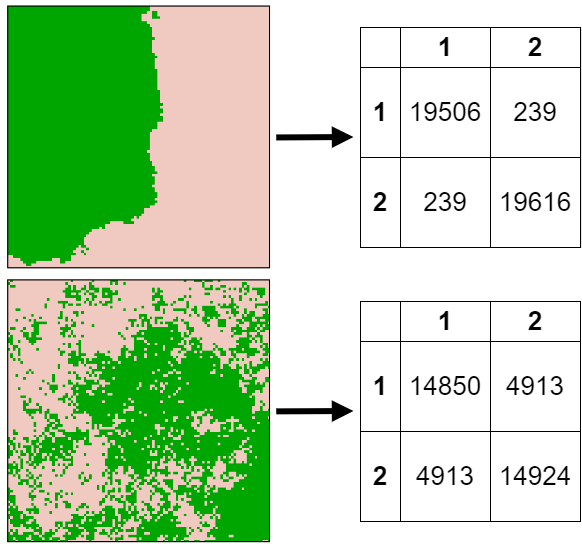
\includegraphics[width=3.64583in,height=3.64583in]{figures/diagram_coma.png}

}

\caption{\label{fig-metody-coma}Przykład dwóch macierzy
współwystępowania dla rastrów o zbliżonej kompozycji i różnej
konfiguracji przestrzennej.}

\end{figure}

Na podstawie macierzy współwystępowania mogą zostać obliczone różne
miary wywodzące się z dziedziny teorii informacji \autocite{nowosad_it}.
Przykładem takiej miary jest entropia brzegowa, która opisuje
zróżnicowanie kompozycji rastra, czyli udziałów każdej z kategorii w
rastrze. Entropia brzegowa może być obliczona zgodnie ze wzorem: \[
H(y) = -\sum_{j=1}^{K}p(y=c_{j})log_2p(y=c_j)
\]

Kolejną miarą jest względna informacja wzajemna. Reprezentuje ona
stopień sąsiadowania ze sobą kategorii w rastrze, czyli jego
konfigurację przestrzenną. Względną informację wzajemną można obliczyć
ze wzoru: \[
U = I(y,x)/H(y)
\] gdzie \(I(y,x)\) oznacza informację wzajemną, liczoną ze wzoru: \[
I(y,x) = H(y) - H(y|x)
\] natomiast \(H(y|x)\) reprezentuje entropię warunkową, obliczaną
zgodnie ze wzorem: \[
H(y|x) = \sum_{i=1}^{K}\sum_{j=1}^{K} p(x=c_i, y=c_j) log_2 p(y=c_i | x=c_j)
\]

W celu porównywania ze sobą sygnatur dwóch rastrów w postaci
dwuwymiarowej macierzy należy je sprowadzić do postaci jednowymiarowego
wektora (histogramu), a następnie przeprowadzić jego normalizację, tak
aby wszystkie wartości sumowały się do 1. Taka postać pozwala na
obliczanie miar odległości lub podobieństwa, pozwalających na
porównywanie histogramów wartości \autocite{Cha2007}. Miary te następnie
pozwalają określić stopień odmienności dwóch rastrów. Podejście to może
być także wykorzystane w innych analizach przestrzennych, jak
wyszukiwanie obszarów o podobnej strukturze przestrzennej, wykrywanie
ich zmian oraz grupowanie obszarów o podobnej strukturze przestrzennej
\autocite{Jasiewicz_GeoPAT,nowosad_motif}.

\hypertarget{sec-pattern-based}{%
\section{Metody analiz różnic pokrycia terenu}\label{sec-pattern-based}}

Zmiany pokrycia terenu w czasie lub różnice w pokryciu terenu pomiędzy
obrazami można analizować przy użyciu wielu metod. Wiele z nich
koncentruje się na analizie różnic na poziomie indywidualnych komórek w
siatce rastra. Najbardziej podstawowym przykładem takiego podejścia jest
analiza ilościowa różnic w pokryciu terenu. Zaletą tego podejścia jest
przede wszystkim łatwość w wykonaniu analizy. Wystarczy zliczyć
wszystkie komórki należące do poszczególnych kategorii dla wybranych
rastrów, a następnie porównać ze sobą te wartości, aby otrzymać wynik
informujący nas o ilościowych różnicach między analizowanymi rastrami.
Analiza ilościowa najczęściej wykorzystywana jest w celu wskazania
ogólnych trendów zmian pokrycia terenu dla określonego obszaru badań jak
na przykład zmniejszanie się obszarów leśnych lub wzrost terenów
zurbanizowanych.

Wszelkie metody analiz zmian pokrycia terenu opierające się na analizie
poszczególnych komórek w siatce rastra są użyteczne na obszarach, gdzie
zmiany między indywidualnymi komórkami dostarczają istotnych informacji.
Ich przydatność jednak maleje, gdy informacja na poziomie pojedynczej
komórki przestaje być tak istotna, na przykład dla rastrów o wysokiej
rozdzielczości lub znacznym zasięgu przestrzennym
\autocite{Jasiewicz_GeoPAT}. W takiej sytuacji bardziej efektywne staje
się zastosowanie metod opartych na analizie struktur przestrzennych
(ang. pattern-based change assessment) \autocite{Netzel2015}.

Pozwalają one przede wszystkim na opis oraz obliczenie podobieństwa
struktur przestrzennych. Głównym zamysłem tych metod jest
przekształcenie danych z postaci dużych rastrów zbudowanych z wielu
indywidualnych komórek zawierających pojedyncze informacje w metryki
krajobrazowe oraz sygnatury przestrzenne, a następnie porównanie ich za
pomocą miar odległości lub niepodobieństwa. Zastosowanie metryk
krajobrazowych w kontekście kompleksowych analiz przestrzennych ma
jednak istotną wadę. Jako że pojedyncza metryka krajobrazowa
reprezentuje wyłącznie jedną, konkretną charakterystykę analizowanego
obszaru, to nie jest w stanie zdefiniować całej charakterystyki
struktury przestrzennej danego rastra. W tym celu korzystniejsze może
okazać się zastosowanie sygnatur przestrzennych. Dzięki temu, że są
dwuwymiarową reprezentacją struktury przestrzennej rastrów, można je ze
sobą porównywać przy użyciu szerokiej gamy istniejących miar odległości
i niepodobieństwa. Umożliwia to także wykonywanie bardziej
skomplikowanych analiz przestrzennych, jak wyszukiwanie, wykrywanie
zmian, grupowanie i segmentacja \autocite{nowosad_motif}.

\hypertarget{miary-odlegux142oux15bci-i-niepodobieux144stwa}{%
\section{Miary odległości i
niepodobieństwa}\label{miary-odlegux142oux15bci-i-niepodobieux144stwa}}

Odległość oraz rozbieżność (inaczej niepodobieństwo) stanowią pewien
policzalny stopień różnorodności pary obiektów. Największą różnicą
między nimi jest to, że odległości są symetryczne, podczas gdy
rozbieżności są niesymetryczne. Oznacza to, że wyłącznie dla miar
odległości otrzymujemy identyczny wynik przy porównywaniu par obiektów A
i B, jak i par B i A.

Niepodobieństwo jest przeciwieństwem podobieństwa. Ponadto, miary
podobieństwa można łatwo przekształcić w miary niepodobieństwa
\autocite{niesterowicz2016}. W związku z tym, w celu uproszczenia
terminologii, wszystkie miary odległości, podobieństwa oraz te wywodzące
się z dziedziny teorii informacji, które zostały wykorzystane w tej
pracy, będą dalej zbiorowo nazywane miarami niepodobieństwa.

Na podstawie podobieństw syntaktycznych, wyróżnia się kilka grup rodzin
miar niepodobieństwa \autocite{Cha2007}: rodzina Minkowski (odległość
euklidesowa, odległość Minkowskiego, odległość Manhattan), rodzina L1
(Canberra, Sorensen, Kulczynski), rodzina Intersection (Intersection,
Wave Hedges, Ruzicka), rodzina Inner Product (Jaccard, Harmonic mean),
rodzina Squared-chord (Fidelity, Matusita), rodzina Squared L2 (Clark,
Pearson X2, Neyman X2), rodzina Shannon's Entropy (Jensen-Shannon,
Kullback-Leibler), a także miary będące połączeniem innych miar (Taneja,
Kumar-Johnson) oraz miary wywodzące się z teorii informacji (informacja
wzajemna, entropia Shannona). Wybór odpowiedniej miary niepodobieństwa
zależy między innymi od rodzaju pomiaru lub sposobu reprezentacji
obiektów \autocite{Cha2007}.

\hypertarget{obliczenie-niepodobieux144stwa-rastruxf3w}{%
\section{Obliczenie niepodobieństwa
rastrów}\label{obliczenie-niepodobieux144stwa-rastruxf3w}}

Pierwszym krokiem, jaki należy podjąć w celu obliczenia podobieństwa
struktur przestrzennych danych rastrowych z wykorzystaniem metod
opartych o sygnatury przestrzenne jest sprowadzenie rastrów wejściowych
do postaci macierzy współwystępowania. Proces utworzenia macierzy
współwystępowania polega na zliczeniu wartości każdej indywidualnej
komórki rastra, a także przylegających do niej komórek (najczęściej
czterech lub ośmiu). Przykładowe macierze współwystępowania widoczne są
na Rycinie \ref{fig-metody-coma}. Następnie, dwuwymiarową macierz należy
sprowadzić do postaci jednowymiarowej, czyli wektora współwystępowania.
Kolejnym etapem analizy jest normalizacja wektora współwystępowania. Po
dodaniu do siebie wszystkich wartości tego wektora powinniśmy otrzymać
wynik równy 1. Po wykonaniu powyższych czynności otrzymujemy
reprezentację rastrów wejściowych, która umożliwia porównanie ich ze
sobą przy użyciu miar niepodobieństwa między rozkładami
prawdopodobieństwa, takich jak rozbieżność Jensena-Shannona. Proces
obliczenia niepodobieństwa dwóch rastrów w postaci schematu przedstawia
Rycina \ref{fig-schemat-porownanie}.

\begin{figure}[t]

{\centering 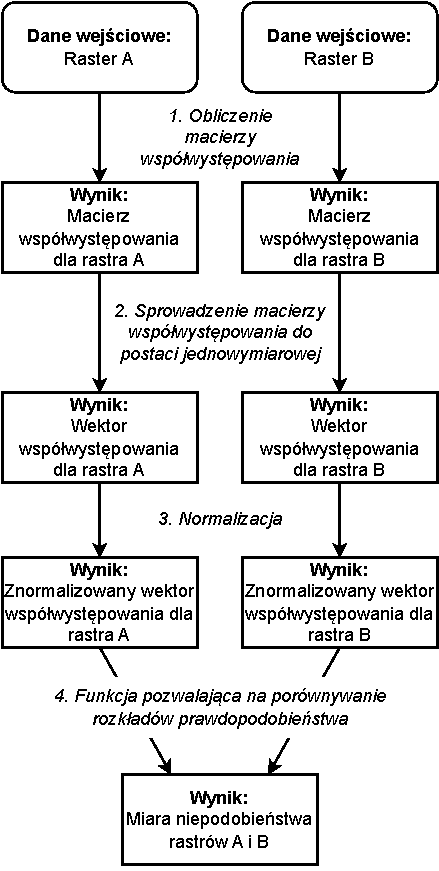
\includegraphics[width=3.125in,height=6.25in]{figures/diagram_raster_comparison.pdf}

}

\caption{\label{fig-schemat-porownanie}Schemat procesu obliczenia
niepodobieństwa dwóch rastrów.}

\end{figure}

\bookmarksetup{startatroot}

\hypertarget{sec-materialy}{%
\chapter{Materiały}\label{sec-materialy}}

W tym rozdziale zostaną omówione najistotniejsze aspekty związane z
formą przeprowadzonej ankiety. W pierwszej kolejności przedstawiony
zostanie proces symulacji rastrów, który został wykorzystany do
stworzenia zbioru danych o określonych parametrach kompozycji i
konfiguracji przestrzennej. Następnie opisany zostanie sposób doboru
odpowiednich pytań do ankiety. W końcowej części rozdziału omówione
zostaną dane przestrzenne o pokryciu terenu CORINE Land Cover, które
zostały wykorzystane do porównania zastosowania wybranych miar
niepodobieństwa w kontekście analiz zmian pokrycia terenu.

\hypertarget{symulowanie-rastruxf3w-o-okreux15blonej-kompozycji-i-konfiguracji-przestrzennej}{%
\section{Symulowanie rastrów o określonej kompozycji i konfiguracji
przestrzennej}\label{symulowanie-rastruxf3w-o-okreux15blonej-kompozycji-i-konfiguracji-przestrzennej}}

Najważniejszym założeniem przy tworzeniu zbioru rastrów do ankiety było
przygotowanie ich w sposób umożliwiający uzyskanie pełnej reprezentacji
wszystkich możliwych wartości kompozycji, jak i konfiguracji
przestrzennej. Zbiór rastrów został przygotowany w języku programowania
R \autocite{R2023}, w oparciu o wykorzystanie funkcji \emph{nlm\_fbm} z
pakietu NLMR \autocite{NLMR2018}. Powyższa funkcja umożliwia uzyskanie
danych rastrowych wypełnionych wartościami zmiennoprzecinkowymi
mieszczącymi się w zakresie od 0 do 1 oraz dowolnymi parametrami
konfiguracji przestrzennej. Funkcja ta pozwala na symulację rastrów przy
użyciu ułamkowych ruchów Browna, będących uproszczeniem ruchów Browna
\autocite{nlm_fbm}. W tej funkcji poziom autokorelacji między kolejnymi
symulacjami jest kontrolowany za pomocą parametru wymiaru fraktalnego
(``fract\_dim''). W kontekście tego badania, parametr ten reguluje
konfigurację przestrzenną. Oznacza to, że w przypadku, gdy
``fract\_dim'' przyjmuje niską wartość, zbliżoną do 0, wartości w
generowanym rastrze rozmieszczone są w sposób losowy, zbliżony do szumu.
Natomiast w przypadku wysokiej wartości ``fract\_dim'', zbliżonej do 2,
na wynikowym rastrze tworzą się skupiska najwyższych i najniższych
wartości, a przejścia pomiędzy nimi mają płynny, wygładzony charakter.

Następnie, aby otrzymać zbiór rastrów uwzględniający także pełen
przekrój kompozycji należy przeprowadzić proces reklasyfikacji rastrów
stworzonych w poprzednim kroku. Procedura ta polega na podziale każdego
dotychczas utworzonego rastra na kategorie pokrycia terenu w różnych
proporcjach, na przykład 90:10, 70:30 oraz 50:50 w przypadku rastrów
zawierających wyłącznie dwie kategorie pokrycia terenu. Wykonanie tego
procesu ułatwia między innymi funkcja \emph{util\_binarize} z pakietu
landscapetools \autocite{NLMR2018}. W tej funkcji proporcje kategorii
pokrycia terenu kontrolowane są za pomocą parametru ``breaks''.
Przykładowo, ustawienie parametru ``breaks'' na poziomie \emph{0.2}
poskutkuje otrzymaniem rastra o kategoriach pokrycia terenu w
proporcjach 20 do 80. Oznacza to, że jedna z kategorii będzie pokrywała
20\% komórek rastra, podczas gdy druga kategoria wypełni pozostałe 80\%
komórek. Na Rycinie \ref{fig-diagram-symulowanie} przedstawiony został
przykład przygotowania rastrów podzielonych na dwie kategorie pokrycia
terenu w sposób opisany powyżej.

\begin{figure}[t]

{\centering 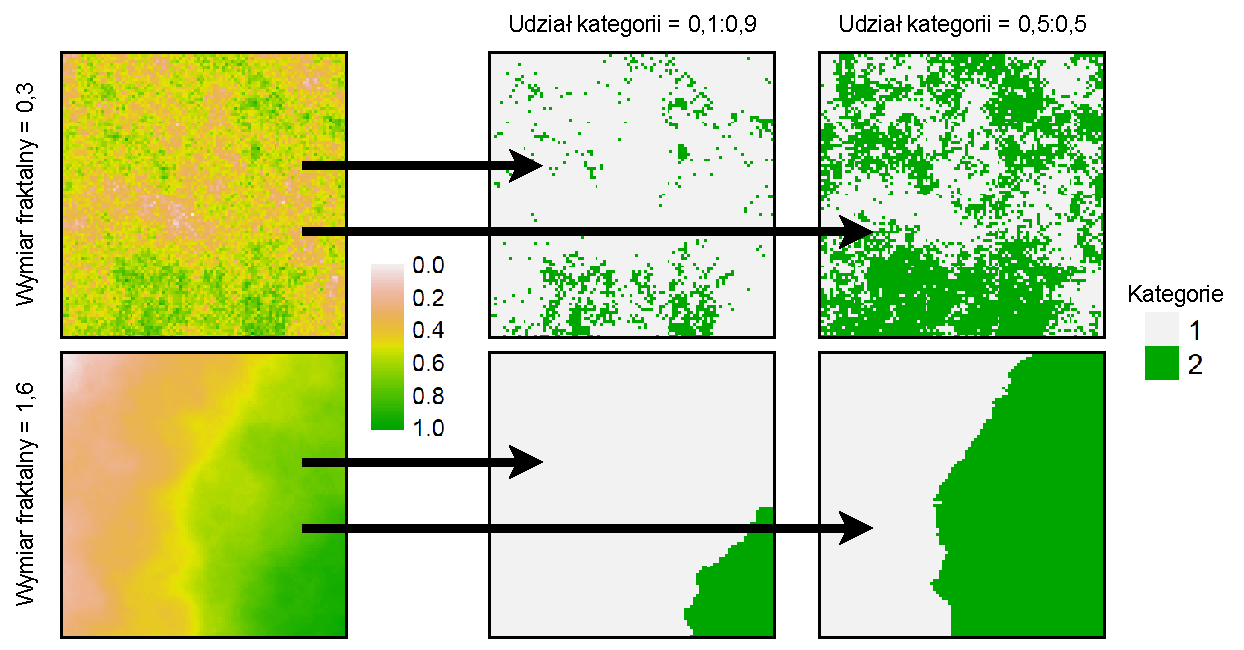
\includegraphics[width=1\textwidth,height=3.22917in]{figures/diagram_rastersim_showcase.pdf}

}

\caption{\label{fig-diagram-symulowanie}Symulowanie rastrów o określonej
kompozycji i konfiguracji przestrzennej}

\end{figure}

Ostatecznie wygenerowane zostały zbiory rastrów składających się
wyłącznie z dwóch lub trzech kategorii pokrycia terenu. Przykład jednego
ze zbiorów rastrów przedstawia Rycina \ref{fig-wykres1_2classes}. Rastry
zawierające trzy kategorie zostały uwzględnione w badaniu w celu próby
wskazania czy liczba kategorii na rastrach ma wpływ na odpowiedzi
udzielane przez ankietowanych.

Po utworzeniu zbioru danych rastrowych bardzo istotne było
potwierdzenie, że obejmuje on pełen zakres rozkładu kompozycji i
konfiguracji. Na potwierdzenie tego założenia pozwoliło obliczenie
wybranych miar opisujących struktury przestrzenne: entropii oraz
względnej informacji wzajemnej.

\begin{figure}[t]

{\centering 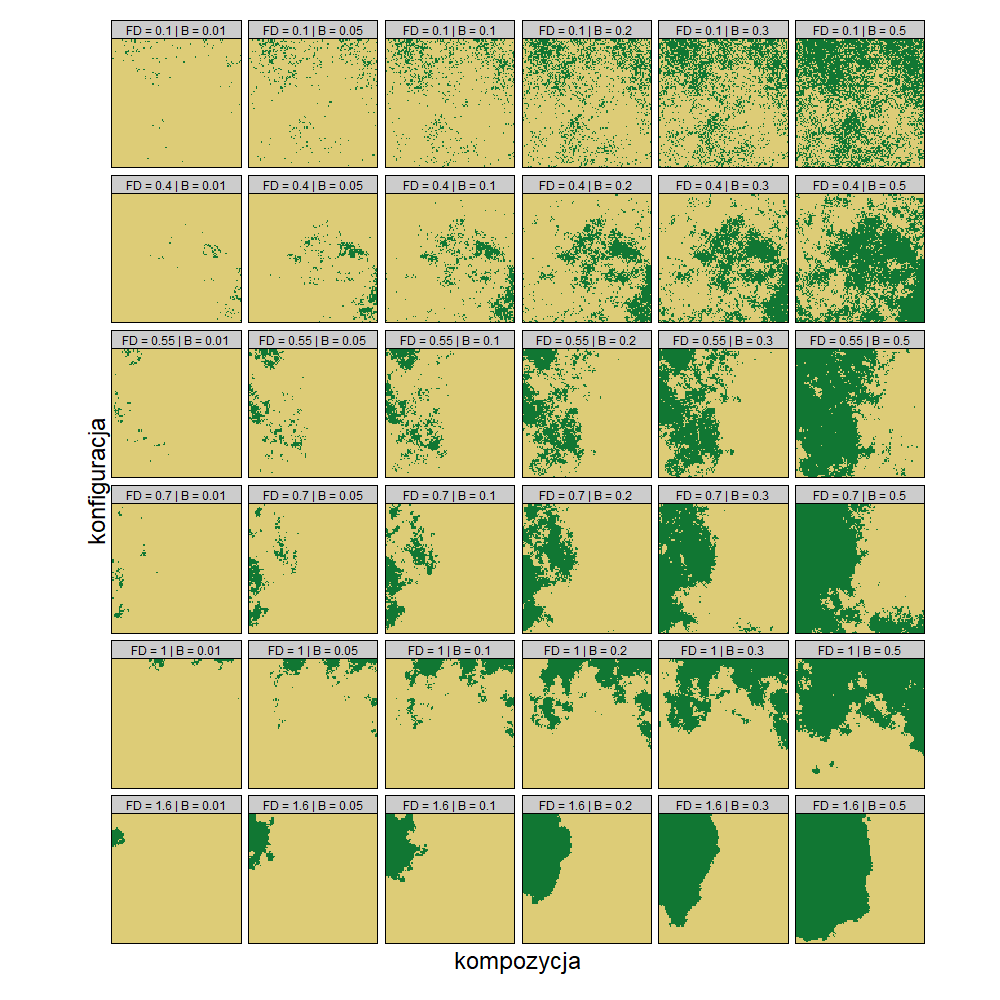
\includegraphics[width=1\textwidth,height=5.72917in]{figures/wykres1_2classes.png}

}

\caption{\label{fig-wykres1_2classes}Przykład zbioru wygenerowanych
rastrów (2 kategorie pokrycia terenu)}

\end{figure}

\hypertarget{sec-przygotowanie1}{%
\section{Przygotowanie ankiety}\label{sec-przygotowanie1}}

Ostatnim krokiem przygotowania danych do ankiety było wybranie par
rastrów tworzących poszczególne pytania tak aby uwzględniały one
wszelkie możliwe różnice struktury przestrzennej rastrów. W tym celu,
pytania w ankietach podzielone zostały na dwie grupy, wewnątrz których
znalazły się po trzy podgrupy pytań.

W pierwszej kolejności respondenci zetknęli się z 24 pytaniami
dotyczącymi rastrów uwzględniających wyłącznie dwie kategorie pokrycia
terenu, a następnie z 24 pytaniami uwzględniającymi trzy kategorie
pokrycia terenu. Pierwsza podgrupa pytań (6 par rastrów) składała się z
par rastrów różniących się między sobą wyłącznie entropią. Podgrupa
druga (6 par rastrów) zawierała wyłącznie rastry różniące się względną
informacją wzajemną. Ostatnia podgrupa (12 par rastrów) składała się z
pytań zróżnicowanych zarówno pod względem entropii, jak i względnej
informacji wzajemnej.

Taki sposób doboru pytań pozwolił na zredukowanie liczby odpowiedzi
wymaganych od respondentów, jak i ograniczenie wpływu błędu selekcji,
który powstałby w wyniku niewłaściwego doboru pytań. Respondenci celowo
nie zostali poinformowani o występujących różnicach pomiędzy kolejnymi
pytaniami, ponieważ mogłoby mieć to wpływ na udzielane przez nich
odpowiedzi, co z kolei mogłoby wpłynąć na ostateczne wyniki badania.

\hypertarget{sec-CLC}{%
\section{Dane CORINE Land Cover}\label{sec-CLC}}

Jednym z etapów porównania miar niepodobieństwa była eksploracja wyników
tych miar przy zastosowaniu w analizie zmian pokrycia terenu na
podstawie danych CORINE Land Cover (CLC). Dane CLC reprezentują
szczegółowe informacje o pokryciu terenu, klasyfikując obszary
geograficzne według różnych kategorii, takich jak lasy, tereny rolnicze,
obszary zurbanizowane czy zbiorniki wodne. Stanowią one istotny
instrument w analizie i monitorowaniu zmian środowiska, a także służą
jako narzędzie wspierające procesy decyzyjne na poziomie europejskim.

Zbiory danych przestrzennych CORINE Land Cover stanowią integralną część
programu CORINE (Coordination of Information on Environment),
wprowadzonego przez Komisję Wspólnot Europejskich w 1985 roku. Program
ten został stworzony w celu skoordynowania przedsięwzięć związanych z
gromadzeniem i przetwarzaniem informacji na temat stanu środowiska
geograficznego w krajach należących do Wspólnoty Europejskiej oraz
standaryzację tych danych w celu ułatwienia wymiany informacji między
państwami członkowskimi \autocite{Bielecka_Ciolkosz_2004}.

Wyniki programu CORINE są udostępniane w formatach wektorowych ESRI i
SQLite geodatabase oraz formacie rastrowym GeoTiff o rozdzielczości
przestrzennej 100 metrów, co oznacza, że jedna komórka rastra obejmuje 1
hektar powierzchni. Do celów tej pracy, wykorzystane zostały dane CLC
dla lat 1990 i 2018 udostępnione do pobrania w formacie GeoTiff na
witrynie Copernicus Land Monitoring Service
(https://land.copernicus.eu/pan-european/corine-land-cover). Dane te
wykorzystują układ współrzędnych ETRS-LAEA (EPSG:3035).

Dane CLC są zorganizowane na trzech poziomach szczegółowości. Na
najwyższym poziomie tej hierarchii wyodrębniono pięć głównych typów
pokrycia terenu: tereny antropogeniczne, tereny rolne, lasy i ekosystemy
seminaturalne, obszary podmokłe oraz obszary wodne. W celu uproszczenia
analizy wyników, dane zostały poddane reklasyfikacji. W wyniku tego
procesu zredukowano liczbę kategorii pokrycia terenu do wyłącznie dwóch:
lasy i pozostałe obszary.

\bookmarksetup{startatroot}

\hypertarget{sec-wyniki}{%
\chapter{Wyniki}\label{sec-wyniki}}

W tym rozdziale przeprowadzona zostanie analiza i podsumowanie wyników
uzyskanych z ankiety. Wyniki zostaną zestawione z miarami
niepodobieństwa uwzględnionymi w analizie.

W celu zidentyfikowania potencjalnych związków pomiędzy percepcją zmian
w pokryciu terenu przez ludzi a miarami niepodobieństwa, które te zmiany
kwantyfikują przeprowadzona została ankieta. Głównym celem ankiety było
aby uzyskanie wstępnych informacji na temat tego w jaki sposób różnice w
entropii oraz względnej informacji wzajemnej między analizowanymi
rastrami wpływają na subiektywne postrzeganie zmian w pokryciu terenu
przez ludzi.

Badanie było realizowane w terminie od 21 do 24 listopada 2022 roku. Z
uwagi na znaczną liczbę rastrów, które miałyby być przedstawione
ankietowanym w trakcie badania, proces zbierania odpowiedzi respondentów
przyjął formę ankiety online. Pozwoliło to respondentom na wygodny
udział w badaniu przy użyciu komputera lub urządzenia mobilnego.
Kwestionariusz stworzony został w formie aplikacji internetowej za
pomocą języka programowania R, na podstawie pakietów \textbf{shiny}
\autocite*{R-shiny} oraz \textbf{shinysurveys}
\autocite*{R-shinysurveys}. Sama aplikacja umieszczona została na
platformie \emph{shinyapps.io} (https://www.shinyapps.io/).
Przeprowadzenie ankiety w formie online umożliwiło systematyczne
gromadzenie oraz przechowywanie odpowiedzi w formie tabelarycznej,
ułatwiając tym samym dalszą analizę i interpretację danych. Respondenci
stanowili grupę 50 studentów drugiego roku studiów inżynierskich na
kierunku Geoinformacja na Wydziale Nauk Geograficznych i Geologicznych
Uniwersytetu im. Adama Mickiewicza. Wybór tej grupy respondentów
oznacza, że byli oni już zaznajomieni z tematyką tworzenia i analiz map
w formie rastrowej oraz pojęciem zmian pokrycia terenu.

Każdy z ankietowanych otrzymał do wypełnienia jeden z dwóch wcześniej
przygotowanych zbiorów pytań. Każdy ze zbiorów składał się z 48 pytań,
przy czym część pytań między zbiorami się pokrywała. Oznacza to, że
łącznie uzyskano odpowiedzi na 93 unikatowe pytania. W każdym z pytań
zadaniem respondentów było określenie podobieństwa na podstawie dwóch
załączonych rastrów. W ramach badania respondenci mieli możliwość
wyrażania swoich odpowiedzi za pomocą pięciostopniowej skali Likerta
\autocite{likert_scale}, która obejmowała poziomy od ``Brak'' przez
``Bardzo małe'', ``Umiarkowane'', ``Bardzo duże'' aż po ``Pełne''.
Wykorzystanie skali Likerta o nieparzystej liczbie przedziałów,
pozwoliło na zastosowanie przedziału środkowego, którego celem było
reprezentowanie odpowiedzi neutralnych lub trudnych do określenia.
Początkowo, zamiast skali Likerta planowano wykorzystać skalę liczbową,
w zakresie mieszczącym się od 1 do 100, jednakże zrezygnowano z tego
pomysłu, jako że znaczenie wartości na skali liczbowej może być
interpretowane inaczej przez każdego respondenta oraz skala ta nie
pozwala na uwzględnienie wspomnianej wcześniej odpowiedzi neutralnej.
Przykład pytania przedstawionego respondentom ilustruje Rycina
\ref{fig-przyklad_pytania}.

\begin{figure}[t]

{\centering 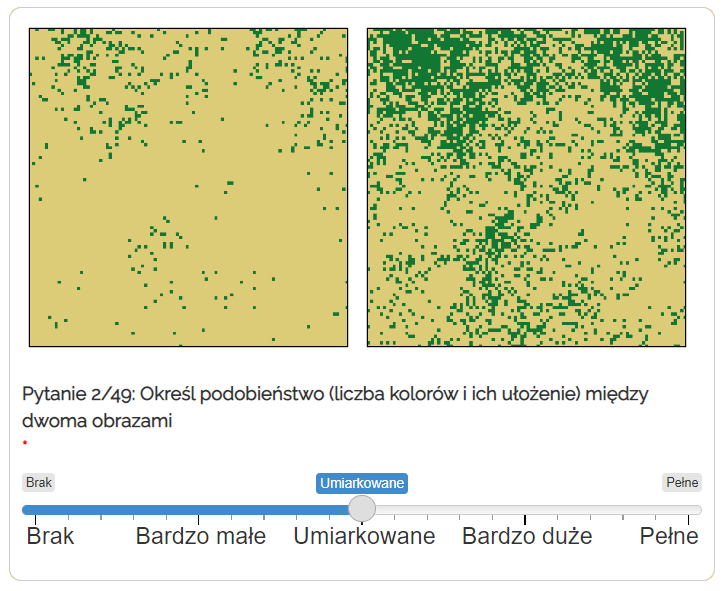
\includegraphics[width=5.10417in,height=4.16667in]{figures/przyklad_pytania.png}

}

\caption{\label{fig-przyklad_pytania}Przykładowe pytanie z ankiety}

\end{figure}

Łącznie uzyskane zostało 2400 odpowiedzi na pytania z ankiety.
Podsumowanie uzyskanych odpowiedzi przedstawione zostało w Tabeli
\ref{tbl-totals_df}. Według ankietowanych prawie 36\% par rastrów
charakteryzowała się brakiem podobieństwa, 32,6\% uzyskanych odpowiedzi
wskazywało na bardzo małe podobieństwo, 18,1\% na umiarkowane, 11,6\%
bardzo duże, natomiast mniej niż 2\% wskazywało na pełne podobieństwo.
Warto tutaj także zwrócić uwagę, że zestawienia wszystkich odpowiedzi w
zależności od liczby kategorii widocznych na rastrach nie wskazują na
znaczące różnice w liczbie odpowiedzi dla danej kategorii. Największą
różnicę stanowi w tym przypadku kategoria ``Bardzo duże'', dla której
liczba odpowiedzi dla rastrów z dwoma i trzema kategoriami pokrycia
terenu różni się zaledwie o 2,7\%. Najmniejszą różnicą charakteryzuje
się kategoria ``Pełne'', gdzie liczba odpowiedzi pomiędzy zestawami
różni się o jedyne 0,9\%.

\hypertarget{tbl-totals_df}{}
\begin{table}
\caption{\label{tbl-totals_df}Podsumowanie odpowiedzi z ankiety }\tabularnewline

\centering
\begin{tabular}{>{\raggedright\arraybackslash}p{3cm}>{\raggedleft\arraybackslash}p{2.5cm}>{\raggedleft\arraybackslash}p{1.5cm}>{\raggedleft\arraybackslash}p{2.5cm}>{\raggedleft\arraybackslash}p{1.5cm}>{\raggedleft\arraybackslash}p{2.5cm}>{\raggedleft\arraybackslash}p{1.5cm}}
\toprule
\multicolumn{1}{c}{Typ odpowiedzi} & \multicolumn{2}{c}{Łącznie} & \multicolumn{2}{c}{Dwie kategorie} & \multicolumn{2}{c}{Trzy kategorie} \\
\cmidrule(l{3pt}r{3pt}){1-1} \cmidrule(l{3pt}r{3pt}){2-3} \cmidrule(l{3pt}r{3pt}){4-5} \cmidrule(l{3pt}r{3pt}){6-7}
 & Liczba odpowiedzi & {}[\%] & Liczba odpowiedzi & {}[\%] & Liczba odpowiedzi & {}[\%]\\
\midrule
Brak & 862 & 35.9 & 420 & 35.0 & 442 & 36.8\\
Bardzo małe & 783 & 32.6 & 398 & 33.2 & 385 & 32.1\\
Umiarkowane & 434 & 18.1 & 211 & 17.6 & 223 & 18.6\\
Bardzo duże & 278 & 11.6 & 155 & 12.9 & 123 & 10.2\\
Pełne & 43 & 1.8 & 16 & 1.3 & 27 & 2.2\\
\addlinespace
Suma & 2400 & 100.0 & 1200 & 100.0 & 1200 & 100.0\\
\bottomrule
\end{tabular}
\end{table}

Aby określić jakie odpowiedzi należały do grupy najczęstszych odpowiedzi
dla poszczególnych pytań, obliczona została miara określana dalej
Poziomem zgodności. Poziom zgodności każdego pytania został obliczony
jako stosunek najczęściej udzielonej odpowiedzi względem całkowitej
liczby odpowiedzi udzielonych na to pytanie. Poziomy zgodności
ankietowanych w podziale na rodzaje pytań znajdują się w Tabeli
\ref{tbl-qtype_agree_df1}. Całkowity poziom zgodności ankietowanych
został oszacowany na 55\%. Oznacza to, że 1321 z 2400 udzielonych
odpowiedzi znalazło się w grupie najczęściej udzielonych odpowiedzi na
pytania. Pytania różniące się zarówno entropią, jak i względną
informacją wzajemną cechowały się najwyższym poziomem zgodności
odpowiedzi wynoszącym 61\%, podczas gdy pytania różniące się wyłącznie
entropią uzyskały wynik 53\%, a pytania różniące się wyłącznie względną
informacją wzajemną uzyskały wynik 52\%.

Najwyższy poziom zgodności odpowiedzi osób ankietowanych wyniósł 92\% i
dotyczył pytania różniącego się zarówno entropią, jak i względną
informacją wzajemną. Aż 24 z 26 osób wskazało na brak podobieństw między
rastrami uwzględnionymi w tym pytaniu. Jest to interesujący wynik,
ponieważ rastry w tym pytaniu wcale nie należały do par rastrów
najbardziej zróżnicowanych pod względem entropii i względnej informacji
wzajemnej. Pierwszy z rastrów charakteryzował się entropią na poziomie
0,08 oraz względną informacją wzajemną wynoszącą 0,09. W przypadku
drugiego rastra, wspomniane wartości wynosiły odpowiednio 0,47 i 0,48.
Oznacza to, że w przypadku obu miar różnica między parami entropii oraz
wynikami względnej informacji wzajemnej wyniosły 0,39.

Najniższy poziom zgodności, czyli zaledwie 38\%, osiągnęło aż 8 pytań.
Wyłącznie dwa z nich dotyczyły pytań zawierających trzy kategorie
pokrycia terenu, podczas gdy pozostałe - dwóch. 75\% z tych pytań
uwzględniało rastry różniące się pod względem względnej informacji
wzajemnej (inna konfiguracja) przy zachowaniu tej samej entropii
(identyczna kompozycja).

\hypertarget{tbl-qtype_agree_df1}{}
\begin{table}
\caption{\label{tbl-qtype_agree_df1}Poziom zgodności ankietowanych w podziale na rodzaje pytań }\tabularnewline

\centering
\begin{tabular}{>{\raggedright\arraybackslash}p{6.5cm}>{\raggedleft\arraybackslash}p{2cm}>{\raggedleft\arraybackslash}p{2cm}>{\raggedleft\arraybackslash}p{2cm}}
\toprule
Rodzaj pytania & Liczba najczęstszych odpowiedzi & Liczba odpowiedzi & Poziom zgodności [\%]\\
\midrule
Różna entropia, różne RMI & 429 & 704 & 61\\
Różna entropia, identyczne RMI & 425 & 796 & 53\\
Identyczna entropia, identyczne RMI & 467 & 900 & 52\\
Łącznie & 1321 & 2400 & 55\\
\bottomrule
\end{tabular}
\end{table}

W kolejnym etapie analizy wyniki uzyskane z przeprowadzonej ankiety
zostały zestawione z wynikami 45 różnych miar niepodobieństwa dla par
rastrów uwzględnionych w ankiecie. Aby ocenić relacje między
najczęstszymi odpowiedziami uczestników ankiety a miarami
niepodobieństwa, przeprowadzono analizę korelacji Spearmana. W ten
sposób uzyskano ranking miar, który został przedstawiony w Tabeli
\ref{tbl-corr_df}.

\hypertarget{tbl-corr_df}{}
\begin{table}
\caption{\label{tbl-corr_df}Zestawienie korelacji miar niepodobieństwa z odpowiedziami ankietowanych }\tabularnewline

\centering
\begin{tabular}{>{\raggedright\arraybackslash}p{4.5cm}rrr}
\toprule
\multicolumn{1}{c}{ } & \multicolumn{3}{c}{Korelacja Spearmana} \\
\cmidrule(l{3pt}r{3pt}){2-4}
Miara niepodobieństwa & Łącznie & Dwie kategorie & Trzy kategorie\\
\midrule
Divergence & -0.46 & -0.45 & -0.63\\
Clark & -0.46 & -0.45 & -0.63\\
Pearson & -0.44 & -0.34 & -0.48\\
Canberra & -0.38 & -0.47 & -0.57\\
Kumar-Johnson & -0.35 & -0.34 & -0.32\\
\addlinespace
Wavehedges & -0.33 & -0.46 & -0.52\\
Inner product & -0.33 & -0.23 & -0.44\\
Additive symmetric chi2 & -0.30 & -0.32 & -0.25\\
Kullback-Leibler & -0.28 & -0.31 & -0.20\\
Taneja & -0.28 & -0.30 & -0.23\\
\addlinespace
Jeffreys & -0.25 & -0.30 & -0.18\\
Fidelity & 0.21 & 0.30 & 0.11\\
Bhattacharyya & -0.21 & -0.30 & -0.11\\
Hellinger & -0.21 & -0.30 & -0.11\\
Matusita & -0.21 & -0.30 & -0.11\\
\addlinespace
Średnia & -0.21 & -0.30 & -0.11\\
Jensen-Shannon & -0.19 & -0.28 & -0.10\\
Różnica Jensena & -0.19 & -0.28 & -0.10\\
Średnia harmoniczna & 0.16 & 0.26 & 0.07\\
Squared chi\textasciicircum{}2 & -0.16 & -0.26 & -0.07\\
\addlinespace
Probabilistyczna symetryczna chi2 & -0.16 & -0.26 & -0.07\\
Neyman & -0.14 & -0.18 & -0.05\\
Cosine & -0.05 & 0.16 & -0.25\\
Manhattan & -0.04 & -0.19 & 0.11\\
Sorensen & -0.04 & -0.19 & 0.11\\
\addlinespace
Soergel & -0.04 & -0.19 & 0.11\\
Odległość Kulczyńskiego & -0.04 & -0.19 & 0.11\\
Lorentzian & -0.04 & -0.19 & 0.11\\
Intersection & 0.04 & 0.19 & -0.11\\
Non-Intersection & -0.04 & -0.19 & 0.11\\
\addlinespace
Czekanowski & -0.04 & -0.19 & 0.11\\
Motyka & -0.04 & -0.19 & 0.11\\
Podobieństwo Kulczyńskiego & 0.04 & 0.19 & -0.11\\
Tanimoto & -0.04 & -0.19 & 0.11\\
Ruzicka & 0.04 & 0.19 & -0.11\\
\addlinespace
Hassebrook & -0.04 & 0.14 & -0.20\\
Jaccard & 0.04 & -0.14 & 0.20\\
Dice & 0.04 & -0.14 & 0.20\\
Gower & -0.02 & -0.19 & 0.11\\
Średnia & -0.02 & -0.17 & 0.14\\
\addlinespace
Chebyshev & 0.01 & -0.14 & 0.16\\
Odl. euklidesowa & 0.00 & -0.15 & 0.15\\
Kwadrat odl. euklidesowej & 0.00 & -0.15 & 0.15\\
K divergence & NA & -0.20 & NA\\
Topsoe & NA & -0.28 & NA\\
\bottomrule
\end{tabular}
\end{table}

Spośród wszystkich analizowanych metod obliczania podobieństwa między
parami rastrów, najlepszy wynik korelacji Spearmana z odpowiedziami
ankietowanych osiągnęły ex aequo metody Divergence oraz Clark ze
współczynnikiem korelacji równym -0,46. Do pozostałych miar, które
osiągnęły dosyć wysokie wyniki korelacji i stanowią o znaczącym związku
miar z odpowiedziami należą: Pearson (-0,44), Canberra (-0,38),
Kumar-Johnson (-0,35), Wave Hedges (-0,33), Inner Product (-0,33),
Additive Symmetric \(\chi^2\) (-0,30), Kullback-Leibler (-0,28), Taneja
(-0,28) oraz Jeffreys (-0,25). Wyniki korelacji aż 21 miar mieszczą się
w zakresie od -0,05 do 0,05, co wskazuje na ich bardzo niewielki lub
brak związku z odpowiedziami udzielanymi przez respondentów. Do miar
niepodobieństwa, które uzyskały najniższe współczynniki korelacji
Spearmana należą odległość euklidesowa oraz kwadrat odległości
euklidesowej, dla których wyniosły one 0,00. Wynik ten świadczy o
kompletnym braku związku między wynikami tych miar a odpowiedziami
ankietowanych.

Odpowiedzi ankietowanych z reguły charakteryzują się wyższym
współczynnikiem korelacji z miarami niepodobieństwa obliczonymi dla
pytań dotyczących rastrów uwzględniających wyłącznie dwie kategorie
pokrycia terenu, niż uwzględniających trzy kategorie pokrycia terenu.
Istotny wyjątek stanowią miary, które osiągnęły najlepsze wartości
współczynnika korelacji Spearmana dla wszystkich odpowiedzi, takie jak
metody Divergence oraz Clark, które także ex aequo osiągnęły najlepszy
wynik korelacji z odpowiedziami na pytania z podziałem na trzy kategorie
pokrycia terenu na poziomie -0,63. Najlepszy wynik korelacji Spearmana
dla pytań uwzględniających rastry z dwoma kategoriami pokrycia terenu
osiągnęła miara niepodobieństwa Canberra (-0,47), a następnie Wave
Hedges (-0,46), Divergence (-0,45) i Clark (-0,45).

Do dalszej analizy wybrane zostały 4 miary niepodobieństwa: Divergence,
Clark, Canberra oraz odległość euklidesowa. Trzy pierwsze zostały
wybrane ze względu na to, że osiągnęły najlepsze wyniki w analizie
korelacji Spearmana, natomiast odległość euklidesowa została wybrana w
celu zestawienia z pozostałymi miarami.

Analizując regresje liniowe miar Divergence, Clark oraz Canberra z
najczęstszymi odpowiedziami udzielanymi przez ankietowanych
(-Figure~\ref{fig-top4measures}) można zauważyć wyraźną liniową relację
o podobnym nasileniu zarówno dla pytań uwzględniających dwie jak i trzy
kategorie pokrycia terenu. Tej liniowej relacji nie da się jednak
zauważyć w przypadku odległości euklidesowej. W przypadku pytań z
rastrami uwzględniającymi dwie kategorie pokrycia terenu miara ta
osiągnęła wynik korelacji Spearmana równy -0,15, podczas gdy dla pytań z
rastrami uwzględniającymi trzy kategorie pokrycia terenu wynik ten
wyniósł 0,15. Oznacza to, że przy wzięciu pod uwagę wszystkich pytań,
jej wyniki zestawione z najczęstszymi odpowiedziami ankietowanych mają
charakter zbliżony do szumu.

Przy okazji omawiania wyników korelacji dla odległości euklidesowej
warto wspomnieć, że zarówno odległość euklidesowa jak i kwadrat
odległości euklidesowej osiągnęły dokładnie takie same wyniki korelacji
Spearmana. Może to oznaczać, że podniesienie wyników odległości
euklidesowej do kwadratu nie ma wpływu na ostateczny wynik analizy
korelacji z wynikami ankiety.

\begin{figure}[t]

{\centering 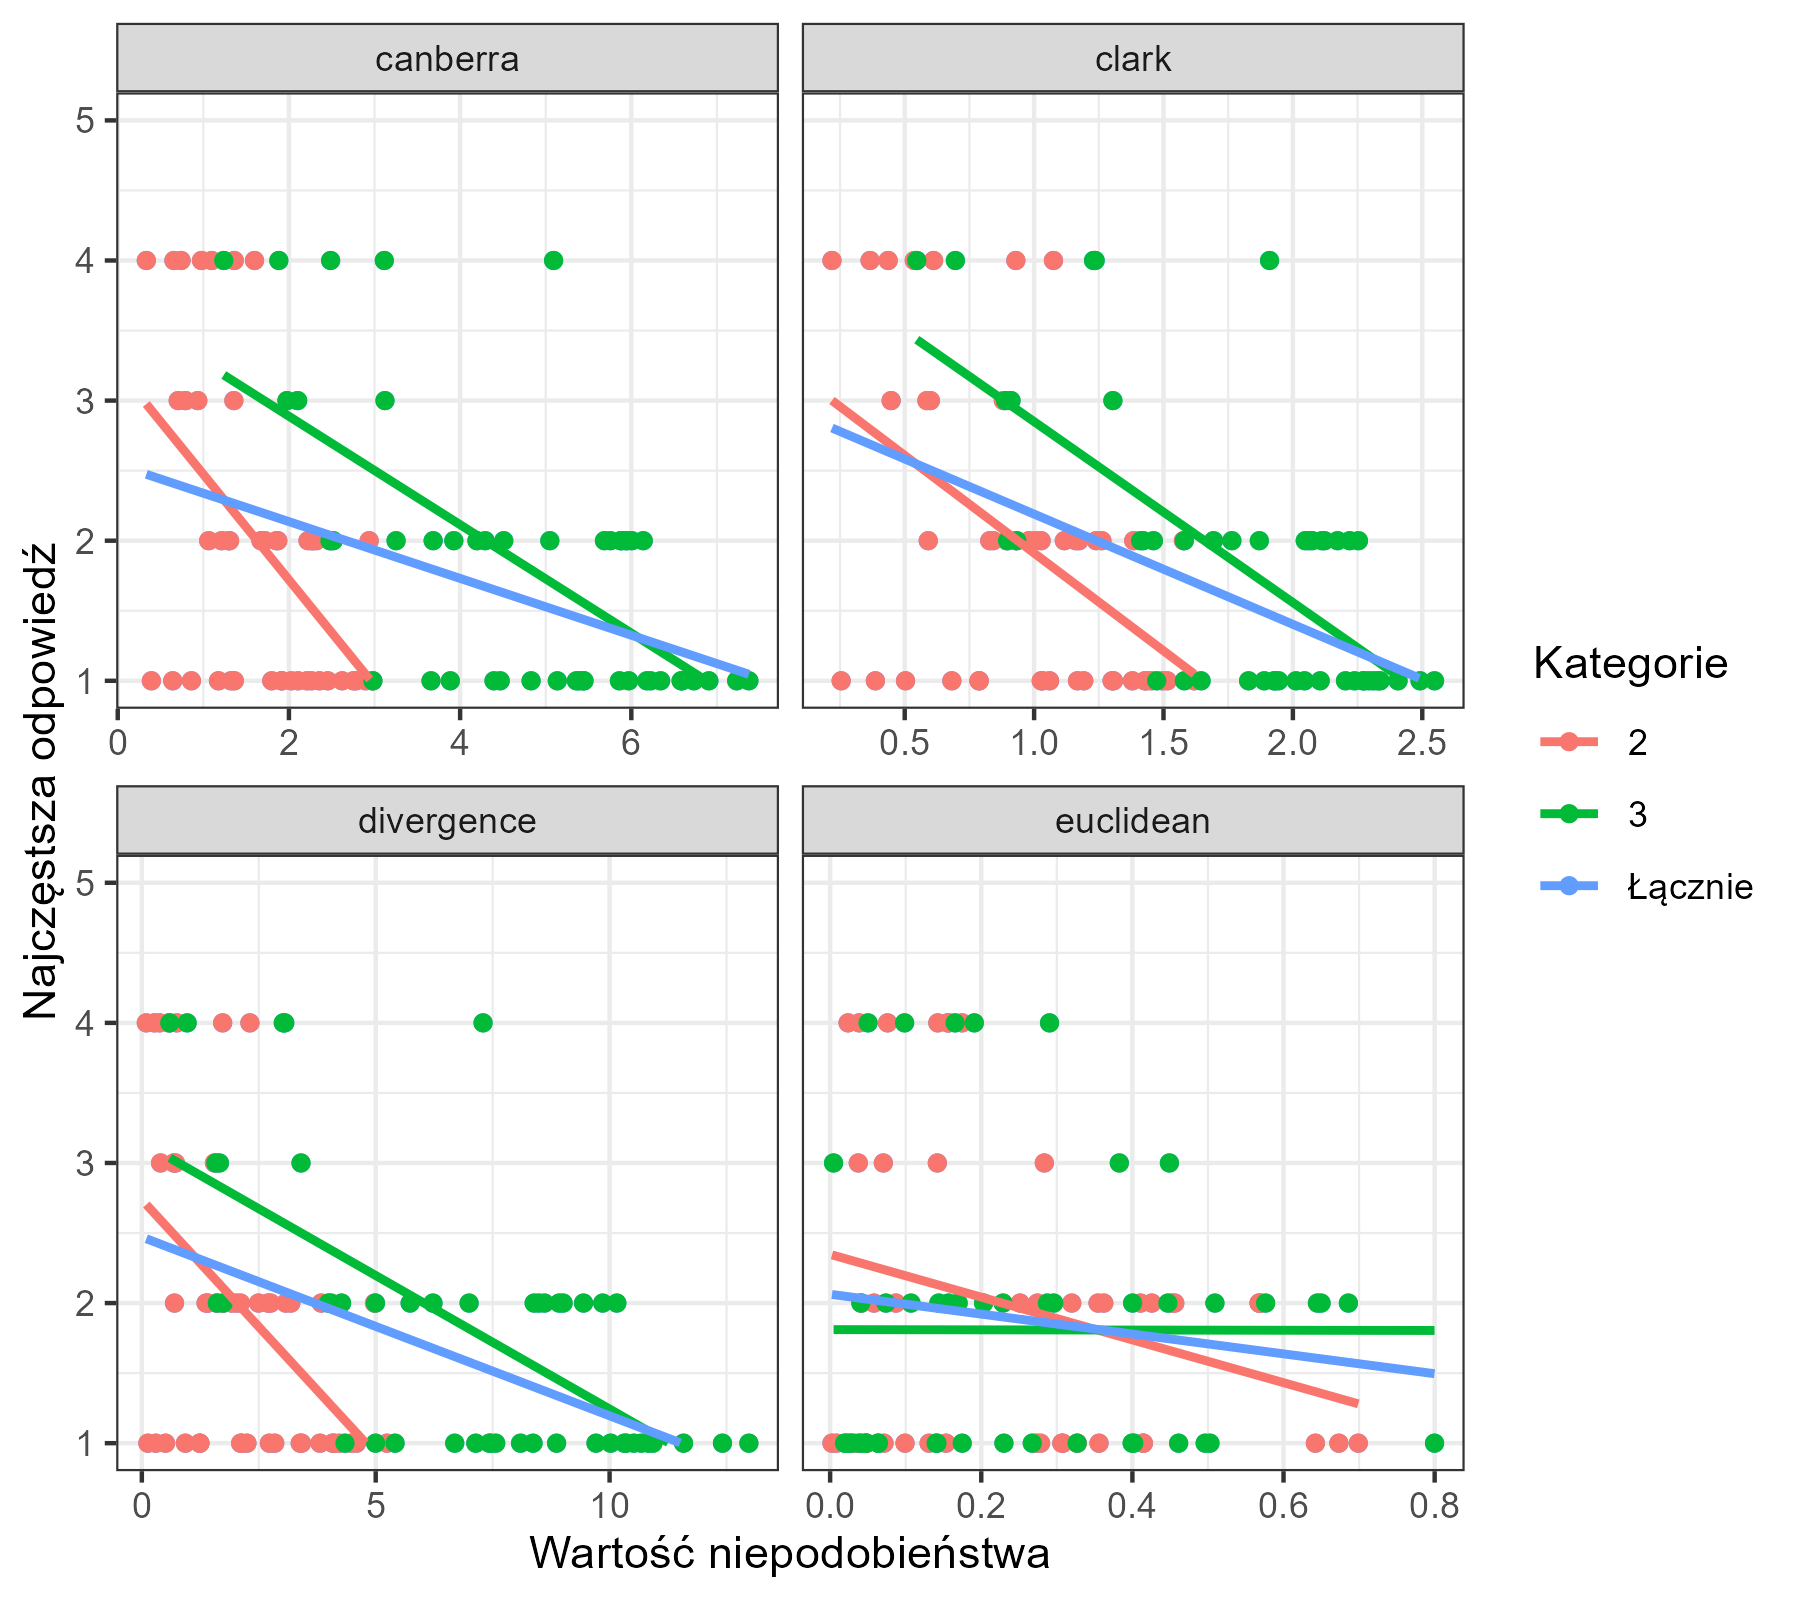
\includegraphics[width=4.6875in,height=4.16667in]{figures/fig-top4measures.png}

}

\caption{\label{fig-top4measures}Regresja liniowa 4 wybranych miar
niepodobieństwa z odpowiedziami ankietowanych}

\end{figure}

Dalsza część porównania wybranych miar niepodobieństwa oparta będzie na
analizie wyników tych miar przy zastosowaniu w analizie zmian pokrycia
terenu na podstawie danych rzeczywistych. W tym celu zostały
wykorzystane dane CORINE Land Cover dla obszaru Polski dla lat 1990 i
2018, które zostały opisane w podrozdziale -Section~\ref{sec-CLC}. Dla
uproszczenia analizy dane CLC zostały zreklasyfikowane tak aby
uwzględniały wyłącznie dwie kategorie pokrycia terenu: lasy i pozostałe
obszary.

Do oceny zmian pokrycia terenu zastosowano metody oparte na analizie
struktur przestrzennych, opisane dokładniej w podrozdziale
-Section~\ref{sec-pattern-based}. Dane wejściowe zostały podzielone na
regularną siatkę kwadratów o wymiarach 100 na 100 pikseli (10 na 10 km).
Następnie, dla tych obszarów obliczone zostały zmiany ich struktur
przestrzennych dla danych z 1990 i 2018 roku wykorzystując do tego
cztery wybrane wcześniej miary niepodobieństwa: Divergence, Clark,
Canberra oraz odległość euklidesowa.

Ze względu na to że oryginalnie wyniki tych miar mieszczą się w różnych
przedziałach wartości, zostały one przeskalowane do zakresu od 0 do 1.
Dzięki temu można łatwiej ze sobą porównać wyniki tych miar. Należy
jednak wziąć pod uwagę, że w takiej sytuacji wartość miar równa 0
niekoniecznie będzie oznaczać całkowity brak zmian w strukturze
przestrzennej, a po prostu najmniejszą zmianę z całego zbioru danych.
Wartość 1 natomiast reprezentować będzie obszary o największej zmianie
struktury przestrzennej.

\begin{figure}[t]

{\centering 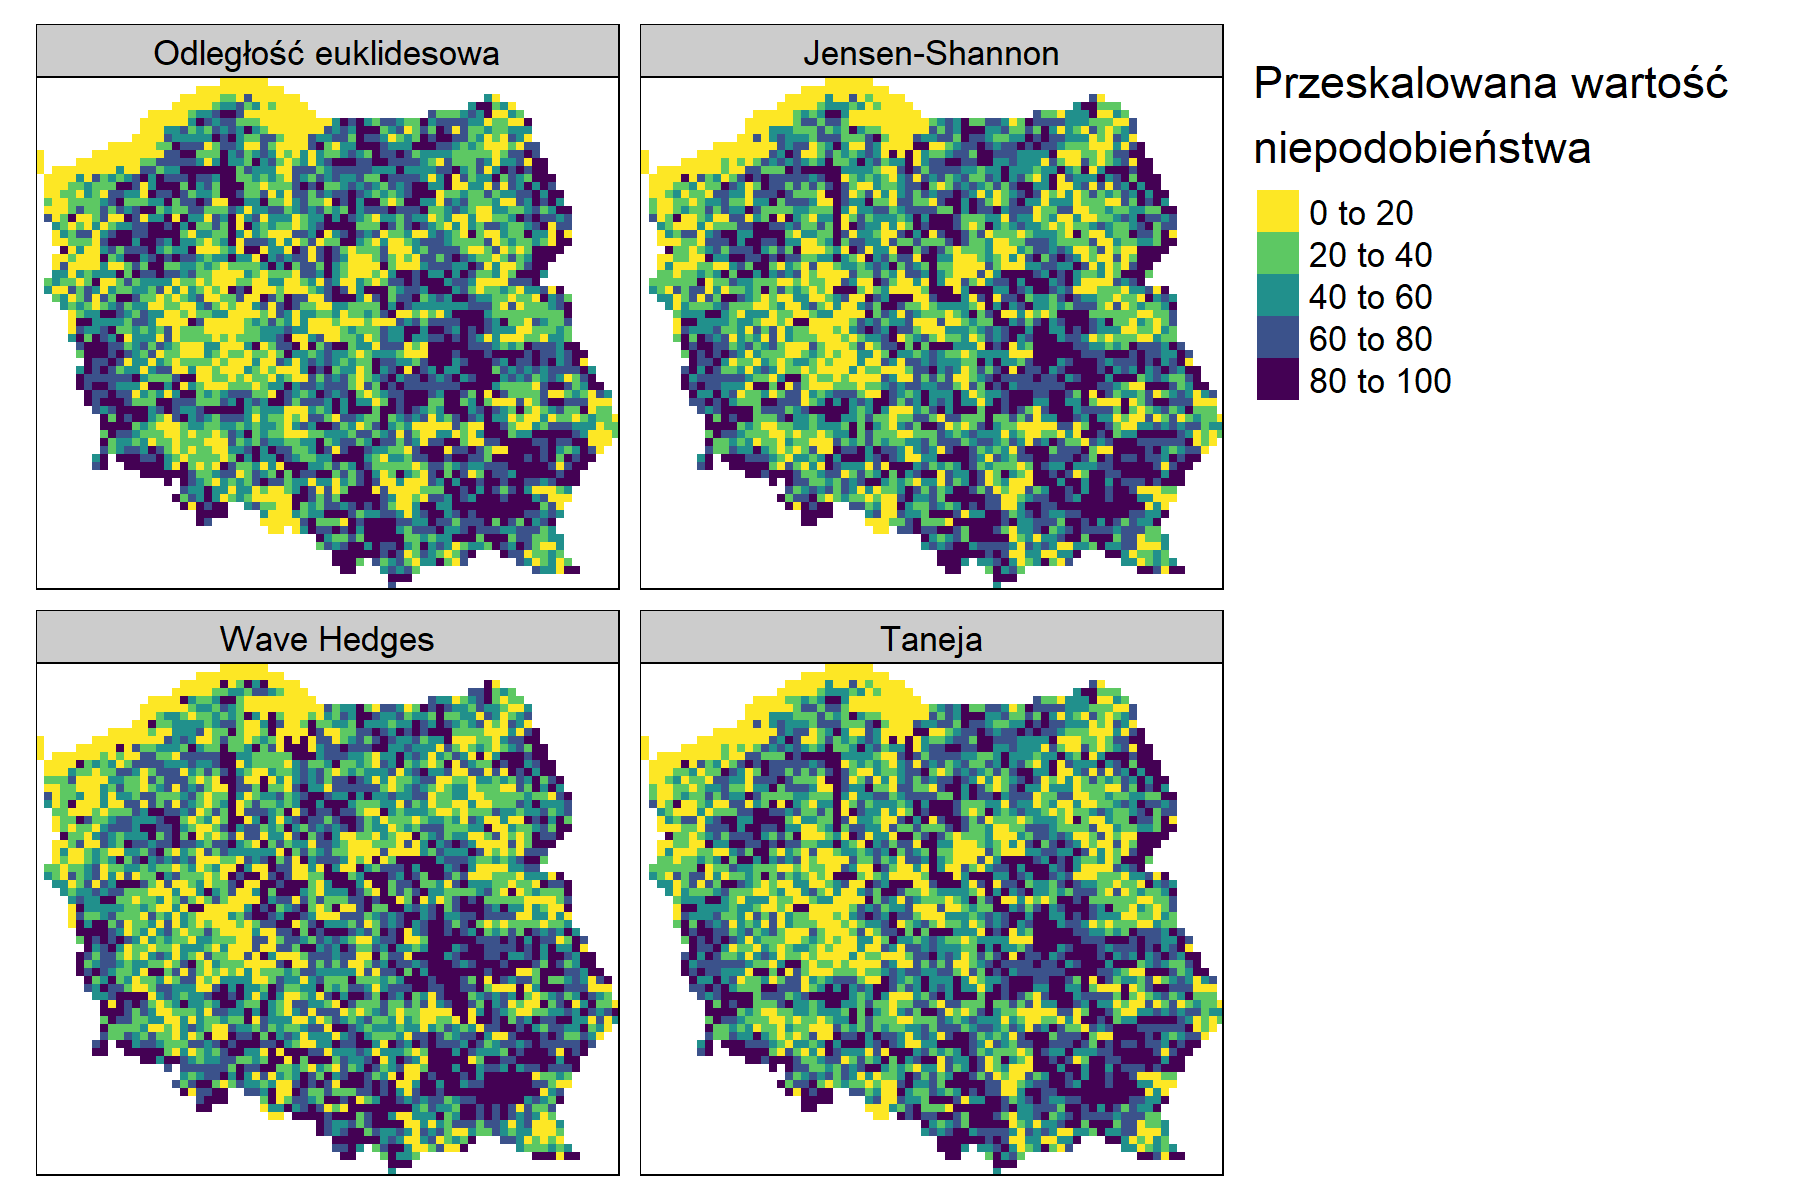
\includegraphics[width=5.83333in,height=4.16667in]{figures/zestawienie_miar1.png}

}

\caption{\label{fig-zestawienie_miar1}Zestawienie map niepodobieństwa
obszarów leśnych dla obszaru Polski dla lat 1990-2018}

\end{figure}

\begin{figure}[t]

{\centering 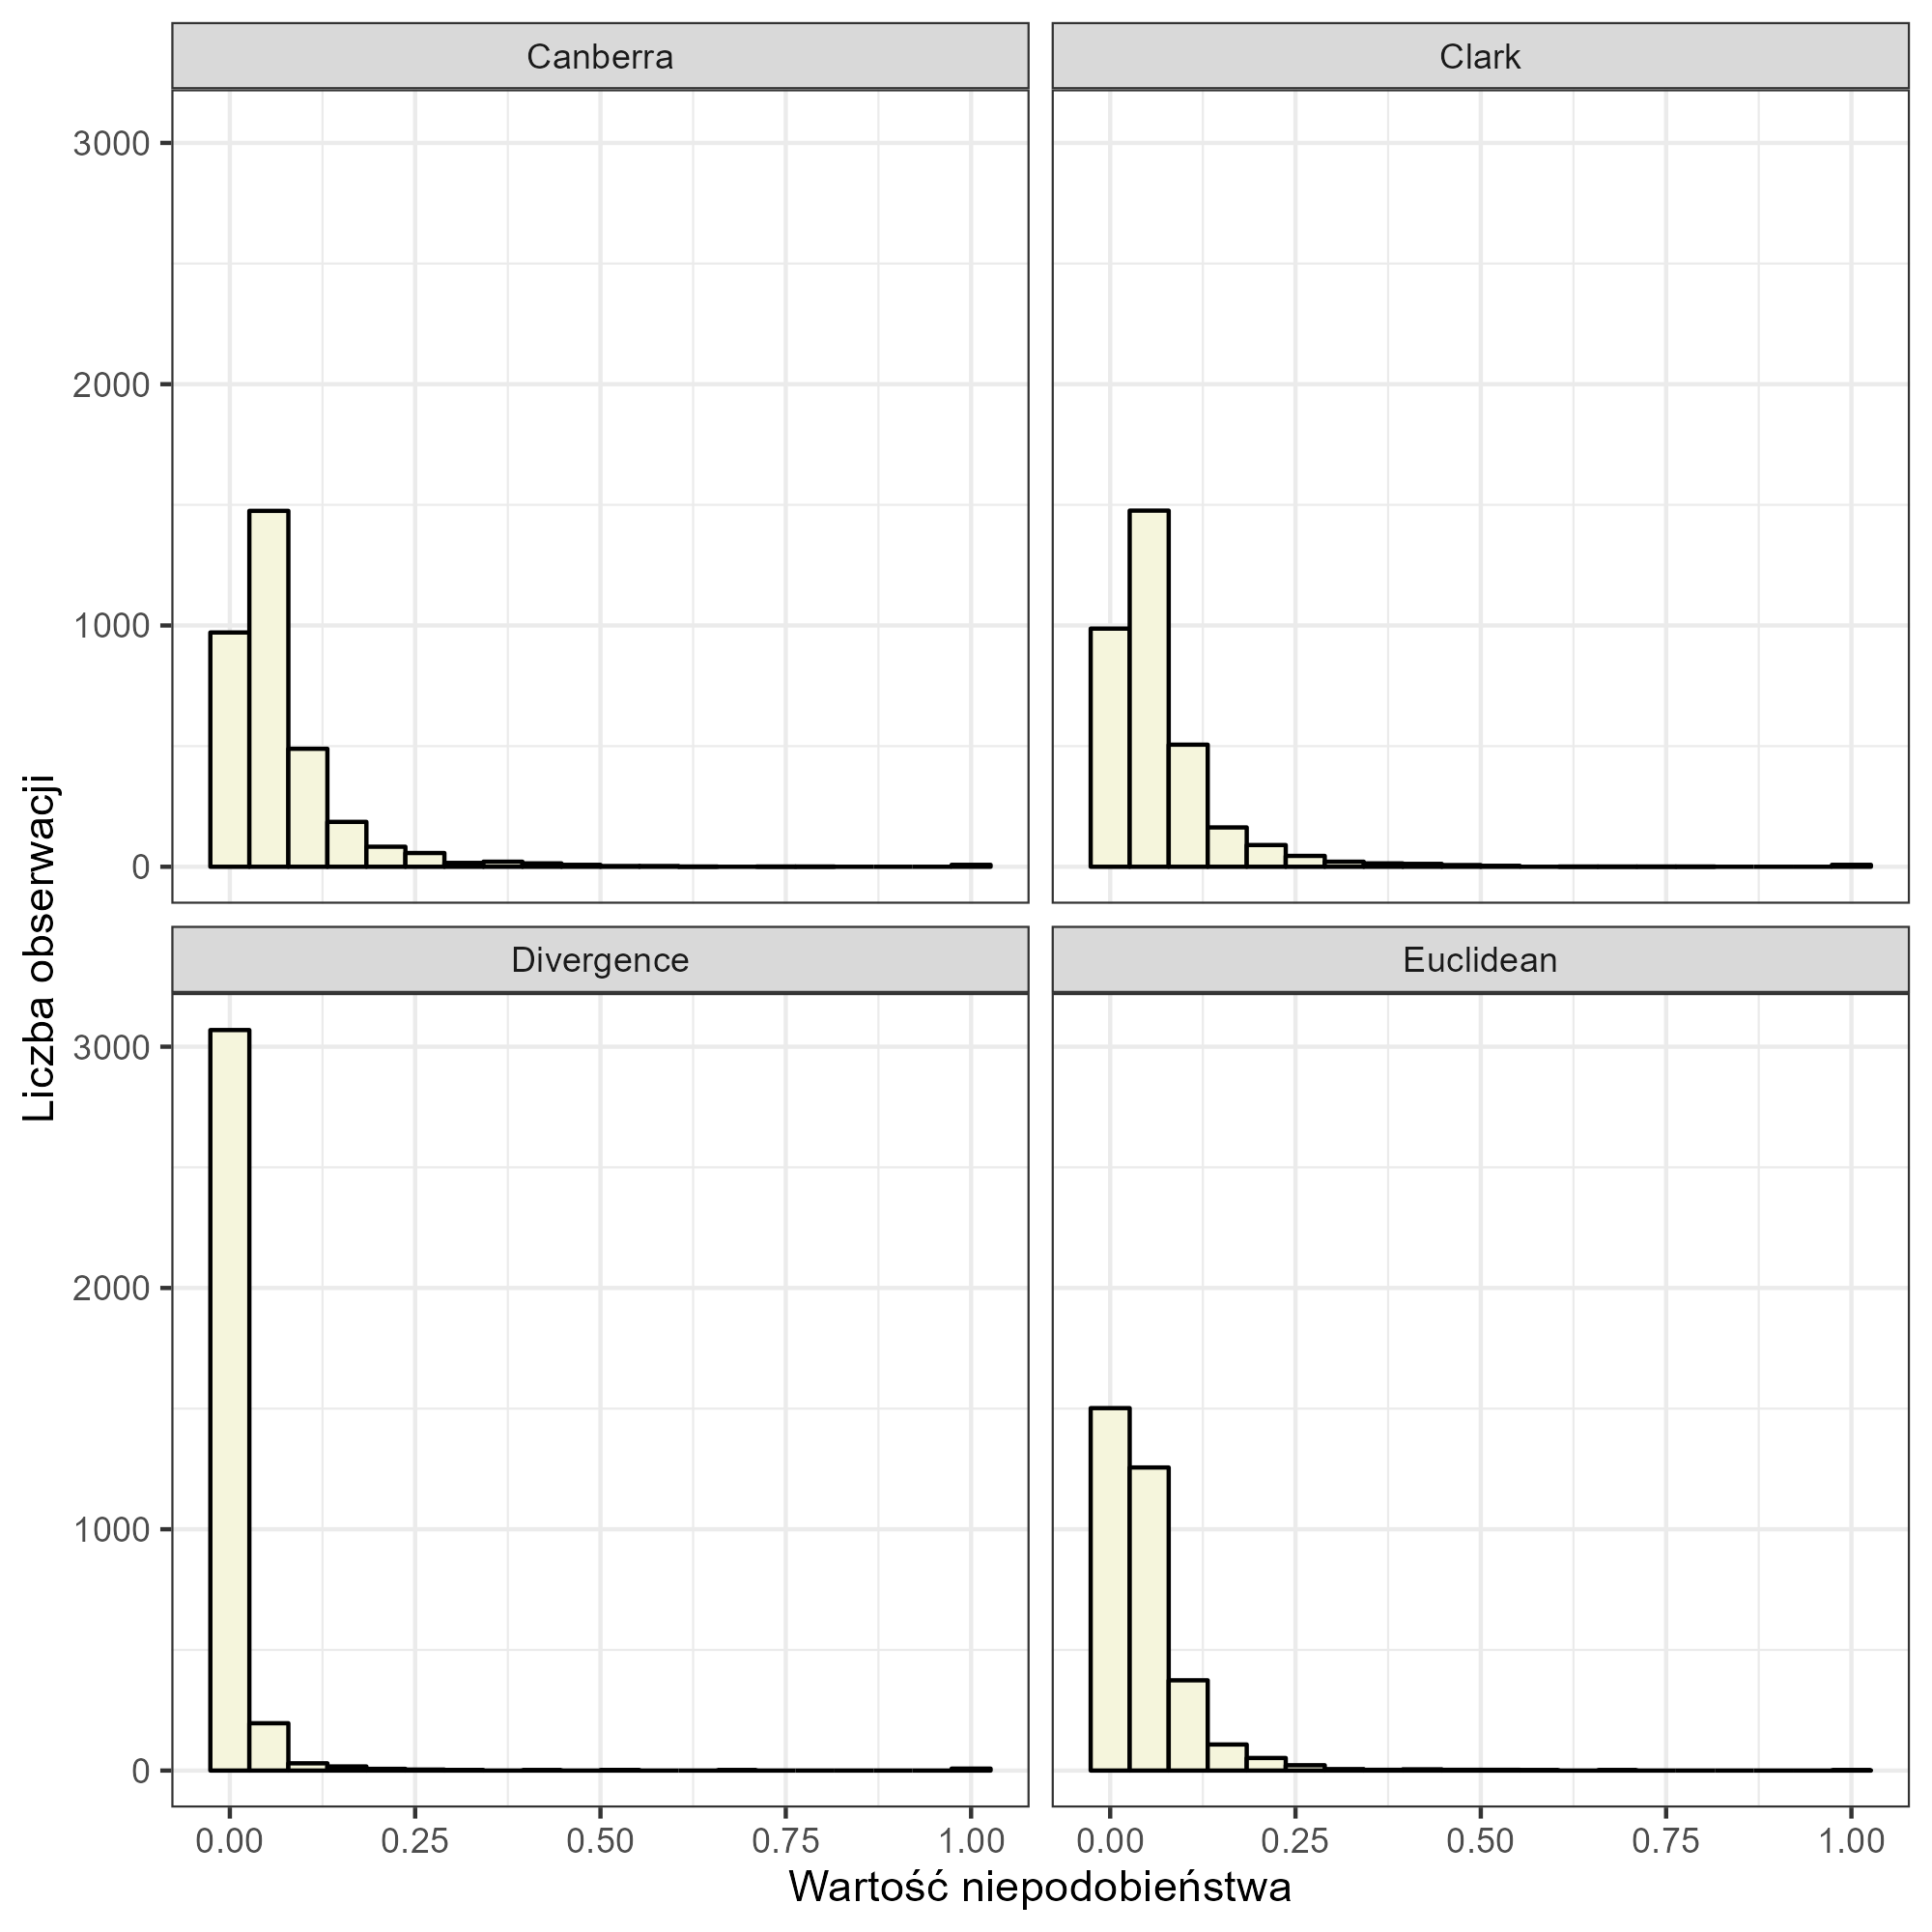
\includegraphics[width=4.16667in,height=4.16667in]{figures/zestawienie_hist1.png}

}

\caption{\label{fig-zestawienie_hist1}Histogramy 4 wybranych miar
niepodobieństwa}

\end{figure}

\hypertarget{tbl-measure_corr_df}{}
\begin{table}
\caption{\label{tbl-measure_corr_df}Zestawienie korelacji między wybranymi miarami niepodobieństwa }\tabularnewline

\centering
\begin{tabular}{>{\raggedright\arraybackslash}p{1.5cm}>{\raggedleft\arraybackslash}p{1.5cm}>{\raggedleft\arraybackslash}p{1.5cm}>{\raggedleft\arraybackslash}p{2cm}>{\raggedleft\arraybackslash}p{2cm}}
\toprule
 & Canberra & Clark & Divergence & Euclidean\\
\midrule
Canberra & 1.00 & 0.99 & 0.83 & 0.54\\
Clark & 0.99 & 1.00 & 0.84 & 0.48\\
Divergence & 0.83 & 0.84 & 1.00 & 0.18\\
Euclidean & 0.54 & 0.48 & 0.18 & 1.00\\
\bottomrule
\end{tabular}
\end{table}

\begin{figure}[t]

{\centering 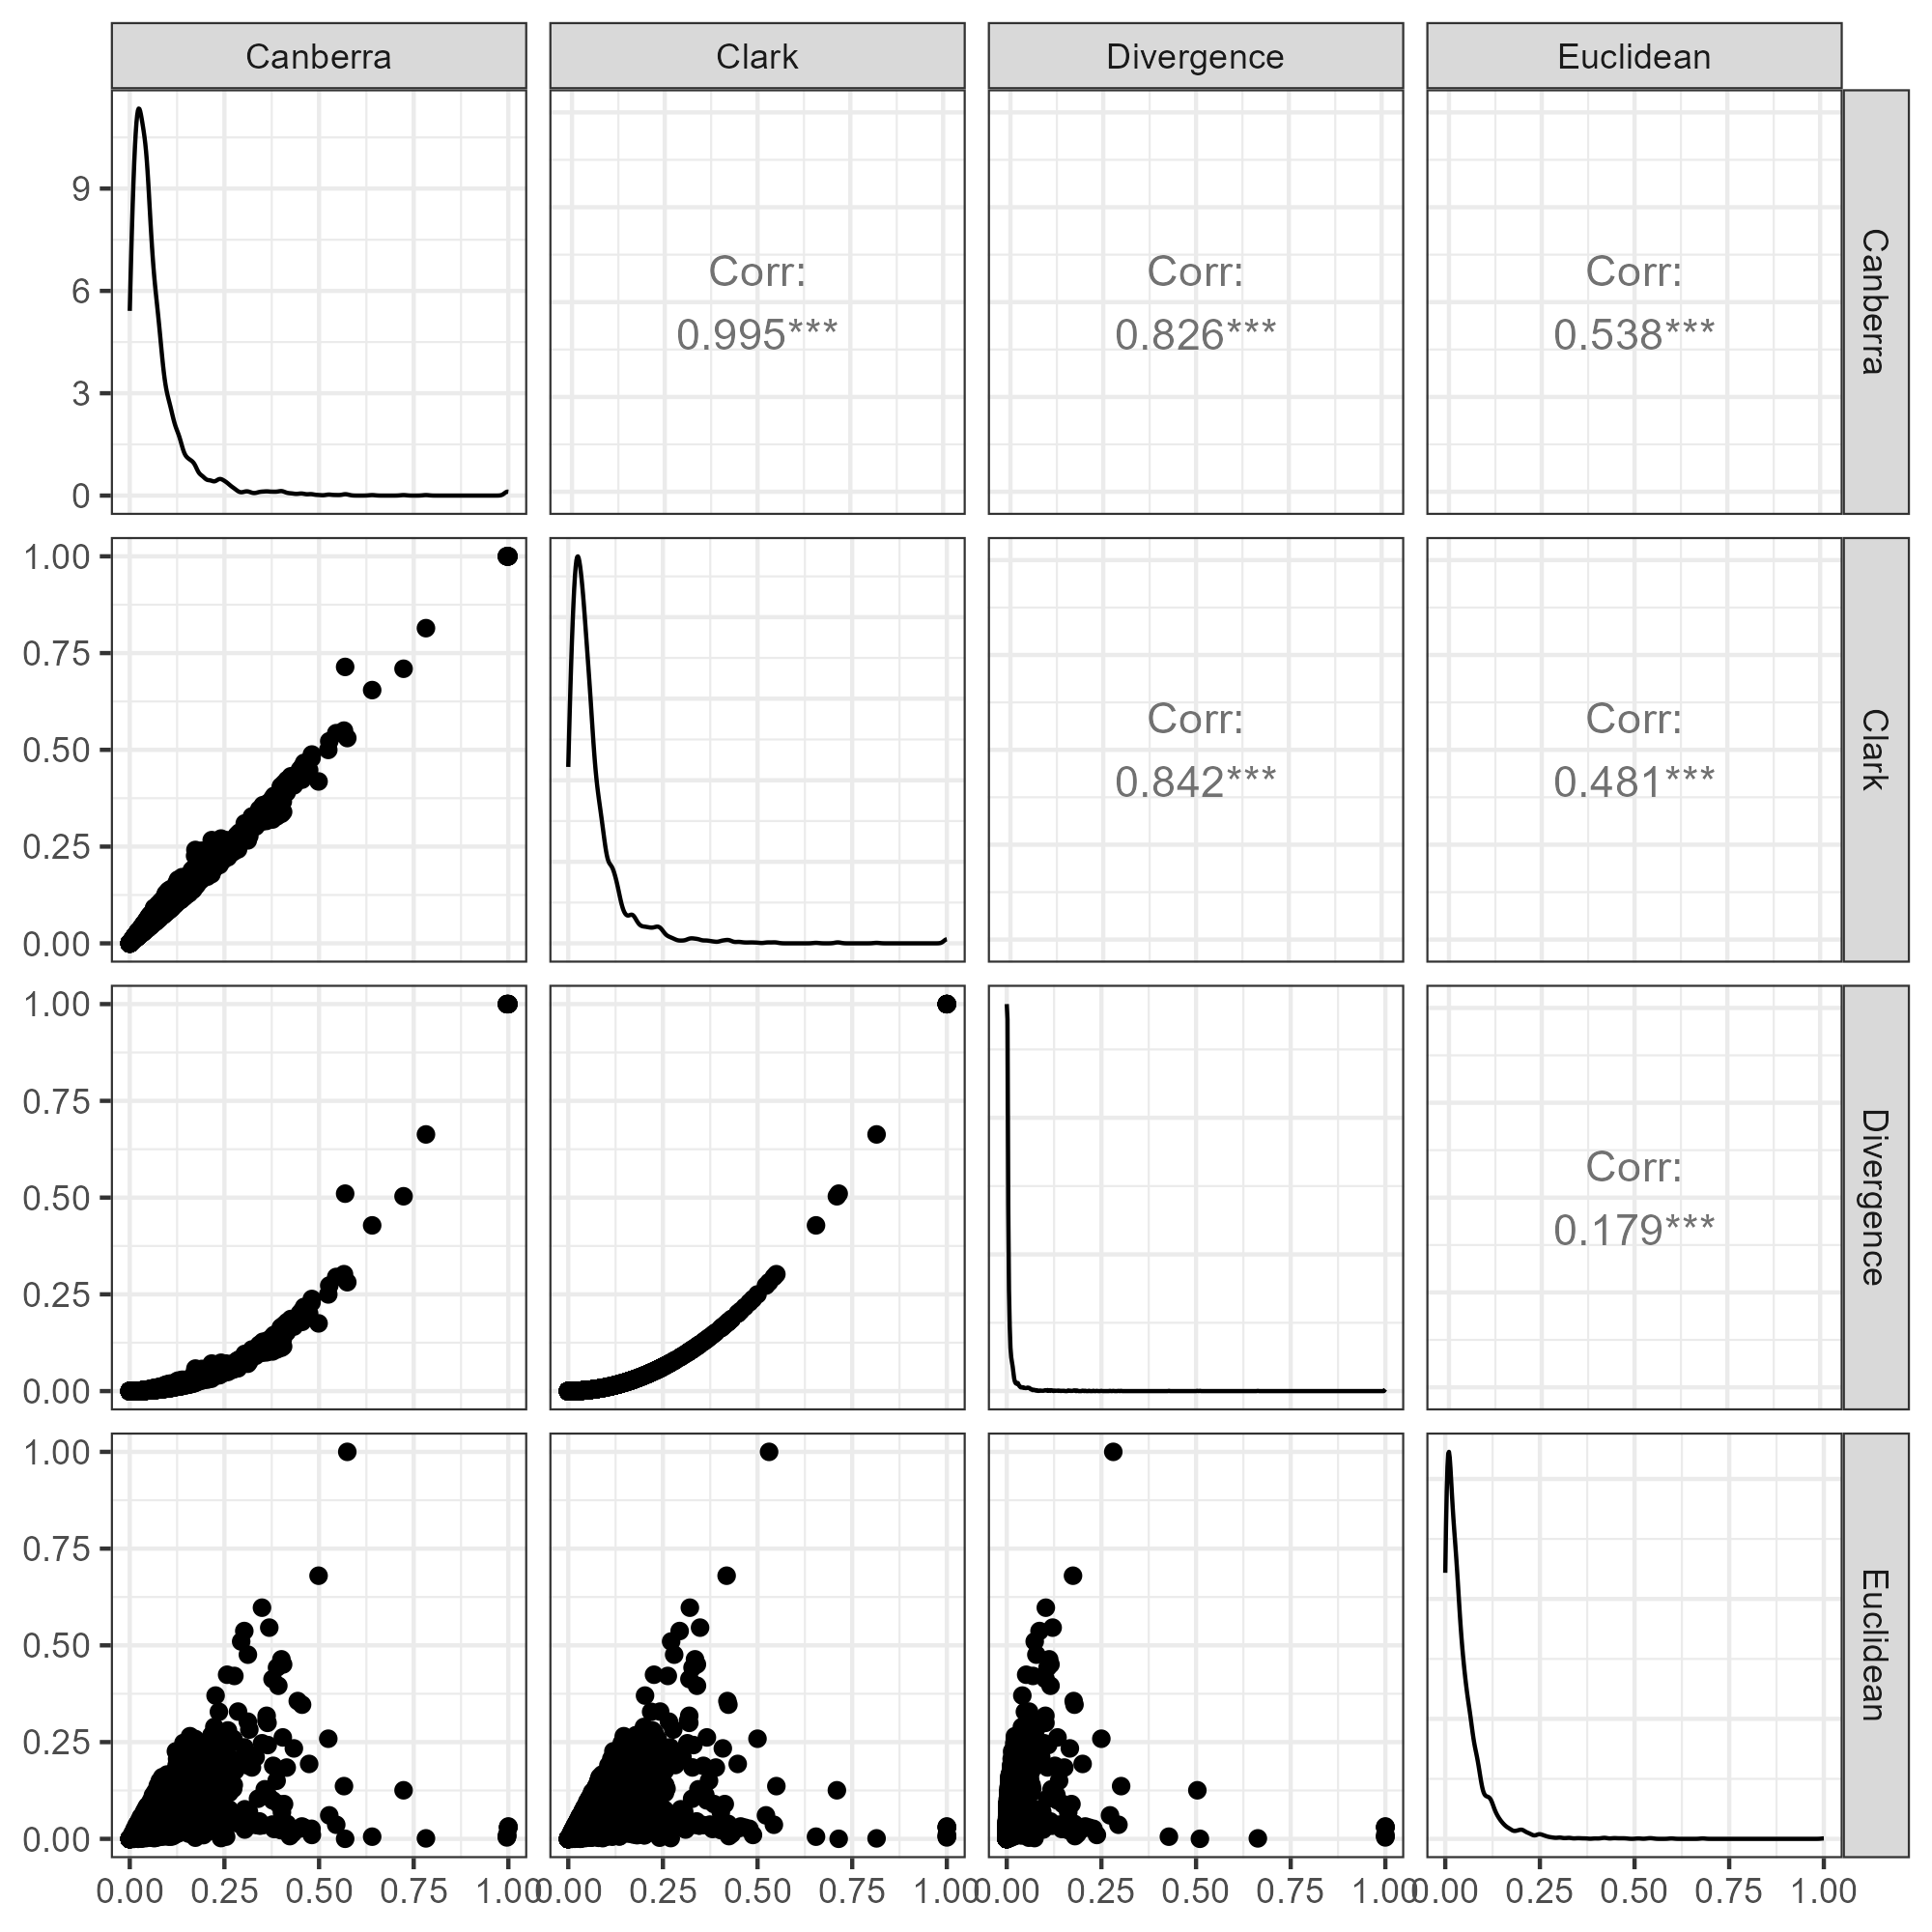
\includegraphics[width=4.16667in,height=4.16667in]{figures/measures_corrplot.png}

}

\caption{\label{fig-measures_corrplot}Regresja liniowa 4 wybranych miar
niepodobieństwa z odpowiedziami ankietowanych}

\end{figure}

\bookmarksetup{startatroot}

\hypertarget{sec-podsumowanie}{%
\chapter{Podsumowanie}\label{sec-podsumowanie}}

\printbibliography[heading=bibintoc, title=Bibliografia]

\end{document}
